\section{Amanzi libraries}

This section describes Amanzi libraries, their limitations and possible 
ways to extend.

\subsection{WhetStone}
This is a low-level library that implements local matrices for various 
discretizations schemes. 
Conceptual desing of the library is presented in Fig.~\ref{whetstone}.

This library contains a factory of discretization scheme that could
be extended by including users schemes.
Example of such an extension is available.


\begin{figure}[h!]
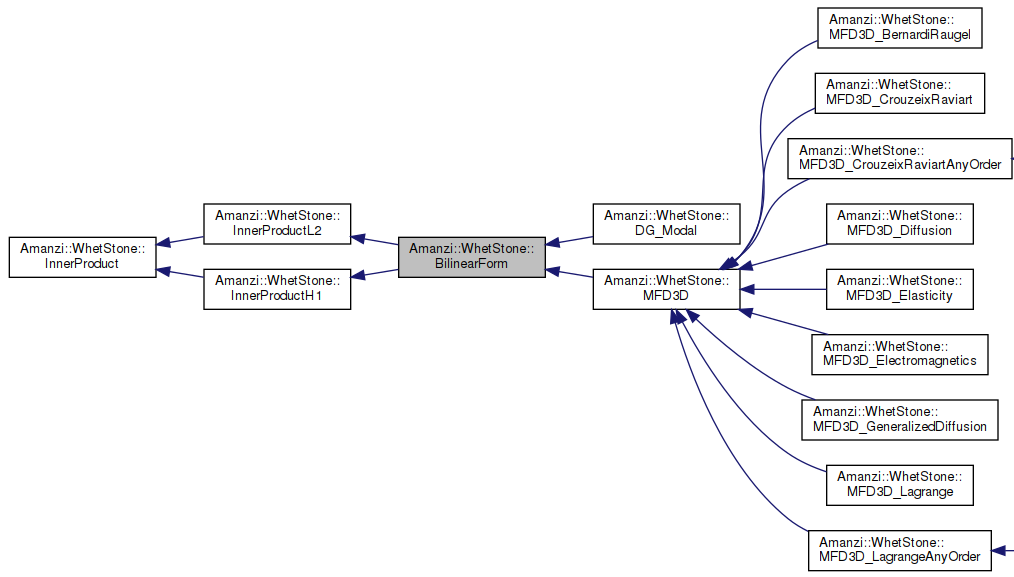
\includegraphics[width=1.0\textwidth]{figs/whetstone.png}
\caption{Schematics\label{whetstone}}
\end{figure}

\subsection{Operators}

Bla-bla-bla

\subsection{PKs}

Bla-bla-bla

